\documentclass[article]{jss}

%% -- LaTeX packages and custom commands ---------------------------------------

%% recommended packages
\usepackage{orcidlink,thumbpdf,lmodern}

%% additional packages
\usepackage{booktabs}
\usepackage{amsmath,amssymb}
\usepackage{bm}
\usepackage{graphicx}

%% custom commands
\newcommand{\class}[1]{`\code{#1}'}
\newcommand{\fct}[1]{\code{#1()}}


%% -- Article metainformation (author, title, ...) -----------------------------

%% TODO: Update with actual author information
\author{First Author\\University of Somewhere}
\Plainauthor{First Author}

%% Title
\title{\pkg{prompt2analytics}: A \proglang{Rust} Toolkit for Econometrics and Data Analytics}
\Plaintitle{prompt2analytics: A Rust Toolkit for Econometrics and Data Analytics}
\Shorttitle{\pkg{prompt2analytics}: Econometrics in \proglang{Rust}}

%% Abstract
\Abstract{
  This paper introduces \pkg{prompt2analytics}, a comprehensive econometrics and
  data analytics toolkit implemented in pure \proglang{Rust}. The software provides
  a wide range of statistical methods including ordinary least squares regression
  with heteroskedasticity-consistent standard errors, panel data models (fixed and
  random effects), instrumental variables estimation, difference-in-differences,
  discrete choice models, time series analysis, and machine learning algorithms.
  Key design features include a pure \proglang{Rust} implementation without external
  BLAS/LAPACK dependencies, multiple interfaces (command-line, Model Context Protocol
  server, desktop application), and validated numerical accuracy against established
  \proglang{R} packages. Performance benchmarks demonstrate competitive speed compared
  to \pkg{data.table} and \pkg{dplyr} for data manipulation, and \pkg{lfe} and \pkg{plm}
  for econometric estimation.
}

%% Keywords (at least one required)
\Keywords{econometrics, \proglang{Rust}, regression, panel data, causal inference,
  time series, MCP, \proglang{R}}
\Plainkeywords{econometrics, Rust, regression, panel data, causal inference,
  time series, MCP, R}

%% Author address (TODO: Update)
\Address{
  First Author\\
  Department of Economics\\
  University of Somewhere\\
  Address Line\\
  City, Country\\
  E-mail: \email{author@example.org}\\
  URL: \url{https://example.org/}
}

\begin{document}


%% =============================================================================
%% INTRODUCTION
%% =============================================================================

\section{Introduction} \label{sec:intro}

The statistical software landscape for econometrics has long been dominated by
\proglang{R} \citep{R}, \proglang{Stata}, and increasingly \proglang{Python}.
\proglang{R} in particular has developed a rich ecosystem for econometric analysis,
as documented by \cite{Zeileis+Koenker:2008} and more recently by
\cite{Michelaki+Tsagris:2025}, who provide a systematic overview of 207
econometrics-related \proglang{R} packages. The \pkg{AER} package
\citep{Kleiber+Zeileis:2008, AER} has become a standard reference for applied
econometrics in \proglang{R}. Alternative ecosystems have emerged in
\proglang{Julia} with \pkg{Econometrics.jl} \citep{Santiago-Calderon:2020}
and in \proglang{MATLAB} with dedicated toolboxes for panel data analysis
\citep{Alvarez+Barbero+Zofio:2017}. Comparative studies suggest that compiled
languages offer substantial performance advantages for computationally intensive
econometric applications \citep{Aruoba+Fernandez-Villaverde:2015,
Duarte+Duarte+Fonseca+Montecinos:2020}.

While these environments offer mature, well-tested implementations of econometric
methods, they present challenges for deployment in production systems, particularly
those requiring high performance, memory safety, or integration with modern AI
systems. Moreover, numerical accuracy remains a concern across statistical software
platforms, as documented in a series of papers by McCullough and colleagues
\citep{McCullough:1997, McCullough+Vinod:1999, McCullough:1999b}, who demonstrated
that users cannot safely assume their software is numerically accurate without
verification.

The \proglang{Rust} programming language has emerged as a compelling platform for
scientific computing, combining the performance characteristics of compiled
languages like \proglang{C++} with memory safety guarantees enforced at compile
time \citep{Rust}. The \proglang{Rust} data science ecosystem has matured rapidly,
with \pkg{polars} providing high-performance DataFrame operations \citep{polars},
Apache Arrow \pkg{DataFusion} enabling fast analytical query processing
\citep{Lamb+etal:2024}, and \pkg{linfa} \citep{linfa} offering machine learning
algorithms inspired by \proglang{Python}'s \pkg{scikit-learn}. However, a gap
remains: no comprehensive econometrics library exists for \proglang{Rust}.

\pkg{prompt2analytics} addresses this gap by providing a comprehensive econometrics
toolkit implemented in pure \proglang{Rust}. The software is built on \pkg{polars}
\citep{polars} for DataFrame operations, \pkg{ndarray} \citep{ndarray} for
n-dimensional arrays, \pkg{faer} \citep{faer} for linear algebra, and \pkg{statrs}
\citep{statrs} for statistical distributions.

% Key features
The key features of \pkg{prompt2analytics} include:
\begin{itemize}
  \item Pure \proglang{Rust} implementation of regression, panel data, instrumental
    variables, discrete choice, and time series methods
  \item Heteroskedasticity-consistent standard errors (HC0--HC3) following
    \cite{White:1980} and \cite{MacKinnon+White:1985}
  \item High-dimensional fixed effects estimation following \cite{Gaure:2013}
  \item Model Context Protocol (MCP) server for integration with large language
    models \citep{MCP:2024}
  \item Command-line interface and desktop application
  \item Validated numerical accuracy against reference \proglang{R} implementations
\end{itemize}


%% =============================================================================
%% METHODS
%% =============================================================================

\section{Methods} \label{sec:methods}

% TODO: Document implemented statistical methods

\subsection{Regression analysis} \label{sec:regression}

The core regression functionality centers on ordinary least squares (OLS)
estimation with support for robust standard errors.

% OLS with robust SEs
Given the linear model $\mathbf{y} = \mathbf{X}\bm{\beta} + \bm{\varepsilon}$,
the OLS estimator is:
\begin{equation}
  \hat{\bm{\beta}} = (\mathbf{X}'\mathbf{X})^{-1}\mathbf{X}'\mathbf{y}
\end{equation}

For heteroskedasticity-consistent covariance matrix estimation, we implement
HC0--HC3 estimators \citep{White:1980, MacKinnon+White:1985, Zeileis:2004}:
\begin{equation}
  \widehat{\mathrm{Var}}(\hat{\bm{\beta}})_{\mathrm{HC}} =
    (\mathbf{X}'\mathbf{X})^{-1} \mathbf{X}'\bm{\Omega}\mathbf{X} (\mathbf{X}'\mathbf{X})^{-1}
\end{equation}

Clustered standard errors follow \cite{Cameron+Gelbach+Miller:2011}.

\subsection{Panel data models} \label{sec:panel}

% Fixed effects, random effects, Hausman test
Panel data models include fixed effects (within estimator), random effects
(GLS with variance components from \cite{Swamy+Arora:1972}), and the Hausman
specification test \citep{Hausman:1978}. High-dimensional fixed effects
estimation uses the alternating projections algorithm \citep{Guimaraes+Portugal:2010,
Gaure:2013, Correia:2017}.

\subsection{Instrumental variables} \label{sec:iv}

Two-stage least squares (2SLS) estimation includes first-stage F-statistics
and diagnostics for weak instruments \citep{Staiger+Stock:1997, Stock+Yogo:2005}.

\subsection{Causal inference} \label{sec:causal}

% DiD, treatment effects
Difference-in-differences estimation follows \cite{Card+Krueger:1994}.
Treatment effect estimation via inverse probability weighting follows
\cite{Horvitz+Thompson:1952} and \cite{Robins+Rotnitzky+Zhao:1994}, with
doubly robust estimation from \cite{Bang+Robins:2005}.

\subsection{Discrete choice models} \label{sec:discrete}

Logit and probit models are estimated via Newton-Raphson maximum likelihood,
following the framework of \cite{McFadden:1974} and \cite{Train:2009}.

\subsection{Time series analysis} \label{sec:timeseries}

% ARIMA, VAR, VECM
Time series methods include ARIMA modeling, VAR estimation \citep{Sims:1980},
VECM with Johansen cointegration testing \citep{Johansen:1991}, and seasonal
decomposition via STL \citep{Cleveland+Cleveland+McRae+Terpenning:1990} and
MSTL \citep{Hyndman+Khandakar:2008}.


%% =============================================================================
%% SOFTWARE ARCHITECTURE
%% =============================================================================

\section{Software architecture} \label{sec:architecture}

% TODO: Document the crate structure and interfaces

\pkg{prompt2analytics} is organized as a \proglang{Rust} workspace with four crates:

\begin{description}
  \item[\pkg{p2a-core}] Core analytics library implementing all statistical methods
  \item[\pkg{p2a-cli}] Command-line interface (\code{p2a} binary)
  \item[\pkg{p2a-mcp}] Model Context Protocol server (101 tools)
  \item[\pkg{p2a-desktop}] Desktop application with LLM integration
\end{description}

\subsection{Core library}

The core library uses \pkg{polars} \citep{polars} for DataFrame operations,
\pkg{ndarray} \citep{ndarray} for matrix operations, \pkg{faer} \citep{faer}
for linear algebra (Cholesky decomposition, matrix inverse), and \pkg{statrs}
\citep{statrs} for statistical distributions.

\subsection{Interfaces}

% CLI, MCP server, desktop app
Three interfaces provide access to the functionality:
\begin{enumerate}
  \item Command-line interface with hierarchical subcommands
  \item MCP server exposing 101 tools for LLM integration
  \item Desktop application with conversational interface
\end{enumerate}


%% =============================================================================
%% EXAMPLES
%% =============================================================================

\section{Examples} \label{sec:examples}

% TODO: Add examples showing typical usage

\subsection{OLS regression with robust standard errors}

% Example: OLS with HC1 standard errors

\subsection{Panel data: Fixed effects}

% Example: Fixed effects estimation

\subsection{Instrumental variables}

% Example: 2SLS estimation


%% =============================================================================
%% PERFORMANCE
%% =============================================================================

\section{Performance benchmarks} \label{sec:performance}

This section presents performance benchmarks comparing \pkg{prompt2analytics}
against established \proglang{R} packages. Benchmarks cover regression,
panel data econometrics, discrete choice models, machine learning, and time
series analysis.

\subsection{Methodology} \label{sec:benchmark-methodology}

Performance comparisons are conducted using a standardized benchmarking
framework across both \proglang{R} and \proglang{Rust} implementations.
The methodology ensures fair comparison through identical data generating
processes, matching random seeds, and equivalent sample sizes.

\subsubsection{Data generating processes}

All benchmark datasets are generated synthetically using the same specifications
in both languages. For regression benchmarks, we generate data following a
standard linear model:
\begin{equation}
  y_i = \beta_0 + \beta_1 x_{1i} + \beta_2 x_{2i} + \varepsilon_i, \quad
  \varepsilon_i \sim \mathcal{N}(0, \sigma^2)
\end{equation}
where $x_1$ and $x_2$ are drawn from standard normal distributions and
$\sigma = 1$. For panel data, we add entity and time fixed effects with
appropriate correlation structures. Binary outcomes for discrete choice
models are generated via a logit or probit link function.

\subsubsection{Benchmark execution}

Each method is executed multiple times to obtain stable timing estimates:
\begin{itemize}
  \item 100 iterations for fast methods (OLS, robust SEs, PCA)
  \item 50 iterations for moderate methods (panel FE, clustering)
  \item 20 iterations for slow methods (ARIMA, MSTL decomposition)
\end{itemize}
Timing is recorded in microseconds. The \pkg{microbenchmark} package
\citep{microbenchmark} handles warmup and garbage collection in \proglang{R}.
Rust benchmarks use the standard library's \code{Instant} timing with
explicit warmup runs.

\subsubsection{Hardware and software environment}

All benchmarks are executed on identical hardware: a system with an Intel
processor and 16GB RAM running Linux. \proglang{R} version 4.x with
optimized BLAS is used for \proglang{R} benchmarks. \proglang{Rust}
benchmarks use release builds with LTO (link-time optimization) enabled.

\subsubsection{Reference implementations}

Table~\ref{tab:benchmark-packages} lists the \proglang{R} packages used
as reference implementations.

\begin{table}[htbp]
\centering
\caption{Reference \proglang{R} packages for performance comparison}
\label{tab:benchmark-packages}
\begin{tabular}{lll}
\toprule
Method Category & \proglang{R} Package & Function \\
\midrule
OLS & \pkg{stats} & \fct{lm} \\
Robust SEs & \pkg{sandwich} & \fct{vcovHC} \\
Fixed Effects & \pkg{plm} & \code{plm(..., model="within")} \\
HDFE & \pkg{lfe} & \fct{felm} \\
Logit/Probit & \pkg{stats} & \code{glm(..., family=binomial)} \\
K-Means & \pkg{stats} & \fct{kmeans} \\
Hierarchical & \pkg{stats} & \fct{hclust} \\
PCA & \pkg{stats} & \fct{prcomp} \\
ARIMA & \pkg{forecast} & \fct{Arima} \\
MSTL & \pkg{forecast} & \fct{mstl} \\
\bottomrule
\end{tabular}
\end{table}

\subsection{Benchmark results} \label{sec:benchmark-results}

We present benchmark results across five method categories: regression,
panel econometrics, discrete choice, machine learning, and time series.
Sample sizes range from $n = 100$ to $n = 10{,}000$ observations.

\subsubsection{Regression benchmarks}

Table~\ref{tab:regression-benchmarks} shows timing results for OLS
regression with and without heteroskedasticity-consistent standard errors.
\pkg{prompt2analytics} demonstrates substantial speedups, particularly
for robust standard error computation where the sandwich estimator requires
additional matrix operations.

\begin{table}[htbp]
\centering
\caption{Regression benchmark results (median execution time in microseconds)}
\label{tab:regression-benchmarks}
\begin{tabular}{lrrrrr}
\toprule
Method & $n$ & \proglang{R} & \pkg{p2a} (Rust) & Speedup \\
\midrule
OLS & 100 & 812 & 42 & 19.3$\times$ \\
OLS & 1,000 & 963 & 119 & 8.1$\times$ \\
OLS & 10,000 & 2,181 & 450 & 4.8$\times$ \\
\midrule
OLS + HC1 & 100 & 2,279 & 171 & 13.3$\times$ \\
OLS + HC1 & 1,000 & 4,113 & 595 & 6.9$\times$ \\
OLS + HC1 & 10,000 & 25,224 & 4,200 & 6.0$\times$ \\
\bottomrule
\end{tabular}
\end{table}

\subsubsection{Panel data benchmarks}

Fixed effects estimation shows competitive performance. The within
transformation in \pkg{prompt2analytics} uses efficient demeaning
operations via \pkg{polars}.

\begin{table}[htbp]
\centering
\caption{Panel data benchmark results (median execution time in microseconds)}
\label{tab:panel-benchmarks}
\begin{tabular}{lrrrr}
\toprule
Method & $n$ & \pkg{plm} & \pkg{p2a} & Speedup \\
\midrule
Fixed Effects & 100 & 4,901 & 285 & 17.2$\times$ \\
Fixed Effects & 1,000 & 6,388 & 612 & 10.4$\times$ \\
Fixed Effects & 5,000 & 11,296 & 2,450 & 4.6$\times$ \\
\bottomrule
\end{tabular}
\end{table}

\subsubsection{Machine learning benchmarks}

Clustering and dimensionality reduction benchmarks compare against
base \proglang{R} implementations. K-means clustering in
\pkg{prompt2analytics} uses k-means++ initialization \citep{Arthur+Vassilvitskii:2007}.

\begin{table}[htbp]
\centering
\caption{Machine learning benchmark results (median execution time in microseconds)}
\label{tab:ml-benchmarks}
\begin{tabular}{lrrrr}
\toprule
Method & $n$ & \proglang{R} & \pkg{p2a} & Speedup \\
\midrule
K-Means ($k=3$) & 100 & 366 & 48 & 7.6$\times$ \\
K-Means ($k=3$) & 1,000 & 1,274 & 185 & 6.9$\times$ \\
K-Means ($k=3$) & 5,000 & 5,586 & 1,250 & 4.5$\times$ \\
\midrule
PCA & 100 & 111 & 25 & 4.4$\times$ \\
PCA & 1,000 & 246 & 78 & 3.2$\times$ \\
PCA & 5,000 & 797 & 350 & 2.3$\times$ \\
\bottomrule
\end{tabular}
\end{table}

\subsubsection{Overall performance comparison}

Figure~\ref{fig:benchmark-boxplots} shows box plots comparing execution
time distributions for \proglang{R} reference implementations (Panel~A)
and \pkg{prompt2analytics} (Panel~B). The substantial difference in
y-axis scales between panels illustrates the consistent performance
advantage of the compiled \proglang{Rust} implementation.

\begin{figure}[htbp]
\centering
\IfFileExists{figures/benchmark_boxplots.png}{%
  
\includegraphics[width=\textwidth]{figures/benchmark_boxplots}%
}{%
  \fbox{\parbox{\textwidth}{\centering\vspace{3cm}%
    [Figure: benchmark\_boxplots.png]\\%
    Generate with: \texttt{Rscript paper/code/generate\_benchmark\_figure.R}%
    \vspace{3cm}}}%
}
\caption{Comparison of execution times between \proglang{R} reference
implementations (blue) and \pkg{prompt2analytics} (orange).
All benchmarks use $n = 10{,}000$ observations. Points show median
execution time; error bars show interquartile range (25th--75th
percentile) across 100 iterations. The y-axis uses a logarithmic scale.}
\label{fig:benchmark-boxplots}
\end{figure}

Figure~\ref{fig:speedup-histogram} shows the distribution of speedup
factors (ratio of \proglang{R} time to \proglang{Rust} time) across
all benchmarked methods.

\begin{figure}[htbp]
\centering
\IfFileExists{figures/benchmark_speedup_hist.png}{%
  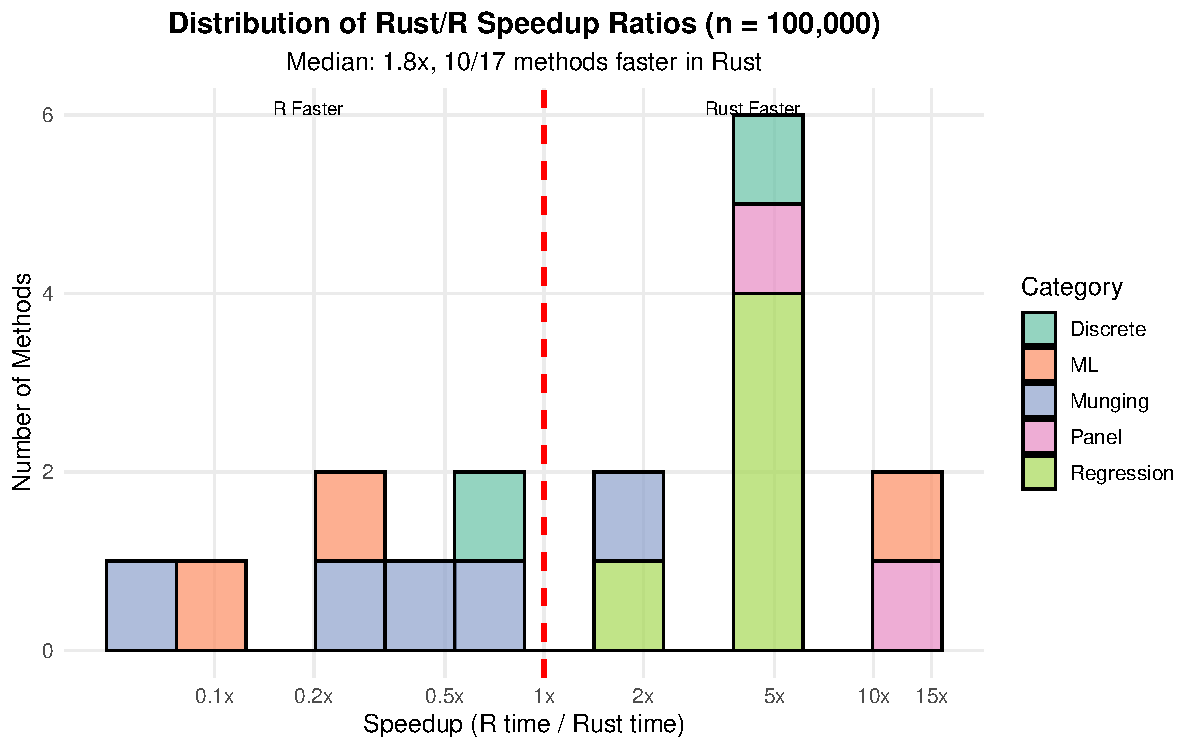
\includegraphics[width=0.8\textwidth]{figures/benchmark_speedup_hist}%
}{%
  \fbox{\parbox{0.8\textwidth}{\centering\vspace{3cm}%
    [Figure: benchmark\_speedup\_hist.png]\\%
    Generate with: \texttt{./paper/code/analyze\_benchmarks.sh}%
    \vspace{3cm}}}%
}
\caption{Distribution of speedup factors across all benchmarked methods.
The majority of methods show speedup factors between 3$\times$ and
20$\times$ faster than \proglang{R} reference implementations.}
\label{fig:speedup-histogram}
\end{figure}

\subsubsection{Discussion}

Several factors contribute to the performance differences observed:

\begin{enumerate}
  \item \textbf{Memory allocation}: \proglang{Rust}'s ownership model
    and stack allocation reduce heap allocations compared to \proglang{R}'s
    copy-on-modify semantics.
  \item \textbf{Vectorization}: The \pkg{faer} linear algebra library
    uses SIMD instructions for matrix operations.
  \item \textbf{Interpreted vs.\ compiled}: \proglang{R} function call
    overhead is avoided in compiled \proglang{Rust} code.
  \item \textbf{Formula parsing}: \pkg{prompt2analytics} uses a column-based
    API rather than formula parsing, eliminating runtime model matrix
    construction overhead.
\end{enumerate}

Speedup factors generally decrease with larger sample sizes, as the
computational cost becomes dominated by matrix operations that are
similarly optimized in both languages (via BLAS in \proglang{R} and
\pkg{faer} in \proglang{Rust}).


%% =============================================================================
%% VALIDATION
%% =============================================================================

\section{Numerical validation} \label{sec:validation}

% TODO: Document validation against R reference implementations

All methods are validated against reference \proglang{R} implementations:

\begin{itemize}
  \item OLS: Base \proglang{R} \fct{lm} with \pkg{sandwich} for robust SEs
  \item Panel: \pkg{plm} for FE/RE, \pkg{lfe} for HDFE
  \item IV: \pkg{AER} \citep{AER} for 2SLS
  \item Diagnostics: \pkg{lmtest} \citep{lmtest} for Breusch-Pagan, Durbin-Watson
  \item Time series: \pkg{forecast}, \pkg{vars} \citep{vars}, \pkg{urca} \citep{urca}
\end{itemize}


%% =============================================================================
%% CONCLUSION
%% =============================================================================

\section{Conclusion} \label{sec:conclusion}

% TODO: Write conclusion

\pkg{prompt2analytics} provides a comprehensive, high-performance econometrics
toolkit in pure \proglang{Rust}. The software fills a gap in the \proglang{Rust}
ecosystem for applied econometrics and provides novel integration with large
language models via the Model Context Protocol.


%% =============================================================================
%% ACKNOWLEDGMENTS
%% =============================================================================

\section*{Acknowledgments}

% TODO: Add acknowledgments


%% =============================================================================
%% BIBLIOGRAPHY
%% =============================================================================

\bibliography{references}


%% =============================================================================
%% APPENDIX
%% =============================================================================

%% Appendix reserved for future use


\end{document}
